\subsubsection{German}%  We consider 4 constructions:
% \begin{inparaenum}[i)]
% \item article-noun gender agreement, possibly with material in the middle,
% \item determiner-noun case concord, again with material in the middle,
% \item preposition case sub-categorization, with material in the middle.
% \end{inparaenum}


\paragraph{Article-noun  gender agreement}
Each German noun belongs to one of three genders (masculine, feminine, neuter), morphologically marked on the article. As the article and the noun can be separated by adjectives and adverbs, we can probe knowledge of lexical gender together with long-distance agreement.
We create stimuli of the form
\exg. \{\underline{der},\ die,\ das\} sehr rote Baum \\
the very red tree \label{ex:german-gender}\\
%    article adverb adjective noun\\
%    `the very red tree'

%\begin{enumerate}[label={(\arabic*)}]
%	\item \begin{tabular}[t]{lllllll}
%	\{\underline{der}, die, das\}& sehr& rote& Baum \\
%	article & adverb & adjective & noun \\
%	the & very & red & tree
%\end{tabular}
%\end{enumerate}
where the correct nominative singular article (\emph{der}, in this
case) matches the gender of the noun.  We then run the CNLM on the
three versions of this phrase (removing whitespace) and record the
probabilities it assigns to them. If the model assigns the highest
probability to the version with the right article, we count it as a
hit for the model. To avoid phrase segmentation ambiguities, we
present phrases surrounded by full stops (see the
\emph{Baum}/\emph{Baumwolle} example above).

%  \cite{de2006generating,mcdonald2013universal}
To build the test set, we select all 4,581 nominative singular nouns
from the German UD treebank (49.3 \% feminine, 26.4 \% masculine, 24.3
\% neuter. OOV noun ratios % \textbf{(how many in total?)}
for WordNLM: 40.0\% for masculine, 36.2\% for feminine, 41.5\% for
neuter). %, and all adjectives from the training set.
We construct four conditions varying the number of adverbs and
adjectives between article and noun.  We first consider stimuli where
no material
intervenes. % \footnote{Due to syncretism in the article paradigm, there is sometimes ambiguity in the choice of the correct article if the noun's morphology does not uniquely indicate that it is a nominative singular from. As this equally affects all feminine nouns, we did not remove such cases. Importantly, this issue is solved as soon as an adjective intervenes, as its form disambiguates case.}
In the second condition, an adjective with the correct case ending,
randomly selected from the training corpus, is added. Crucially, the
ending of the adjective does not reveal the gender of the noun.  We
only used adjectives occurring at least 100 times, and not ending in
-\emph{r}, as the latter often reflect lemmatization
problems.\footnote{TreeTagger occasionally failed to remove the
  inflectional suffix -\emph{r} when lemmatizing.}  We obtained a pool
of 9,742 adjectives to sample from, also used in subsequent
experiments.  74.9\% of these were OOV for the WordNLM.  In the third
and fourth conditions, one (\emph{sehr}) or two adverbs (\emph{sehr
  extrem}) intervene between article and adjective. These do
not cue gender either. We obtained 2,290 (m.), 2,261 (f.), and 1,111 (n.)
stimuli, respectively. We constructed an n-gram baseline picking the
article most frequently occurring before the phrase in the training
data, breaking ties randomly. OOVs were excluded from WordNLM
evaluation, resulting in an easier test for this rival model. However,
here and in the next two tasks, CNLM performance on this reduced set
was only slightly better, and we do not report it here.

Results are presented in Figure \ref{fig:german-syntax}
(left). WordNLM performs best, followed by the LSTM CNLM.  The n-gram
baseline performs similarly to the CNLM when there is no intervening
material, which is expected, as a noun will often be preceded by its
article in the corpus. However, its accuracy drops to chance level
(0.33) in the presence of an adjective, whereas the CNLM is still able
to track agreement. %
% This problem would not be
% mitigated by interpolation with or backoff to lower-order n-grams, as
% the relevant gender information is present only on the first and last
% word of each stimulus. We conclude that, while direct association
% between articles and nouns can be learnt from simple corpus
% statistics, the CNLM has some capability to preserve the relevant
% information across more than a dozen timesteps.
The RNN variant is much worse. It is outperformed by the n-gram model
in the adjacent condition, and it drops to random accuracy as more
material intervenes. We emphasized at the outset of this section that
CNLMs must track agreement across much wider spans than
word-based models. The LSTM ability to preserve information for
longer might play a crucial role here.

% Note that, at the character level, even ``adjacent''
% agreement requires carrying information through multiple time steps
% (the agreement violation will not emerge until enough characters of
% the noun have been processed to disambiguate its gender with respect
% to its prefix-sharing cohort).

% The exclusion of OOVs and thus limiting experiments on word-level models to frequent words might create an unfair advantage; running the CNLM only on those stimuli given to the word-level model results in slightly better accuracies but the same pattern of results.

\begin{figure*}
% 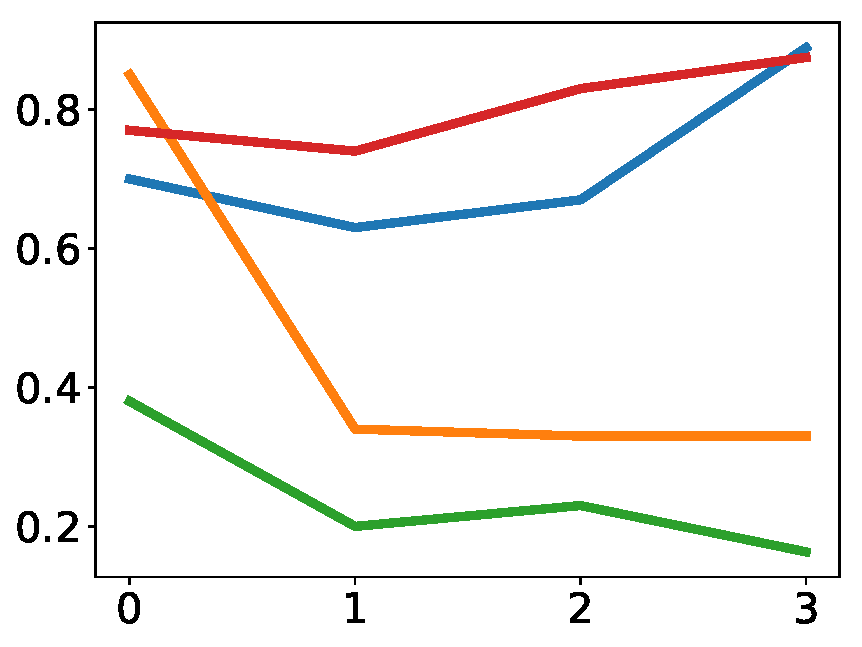
\includegraphics[width=0.24\textwidth]{figures/german-gender-m.pdf}
% 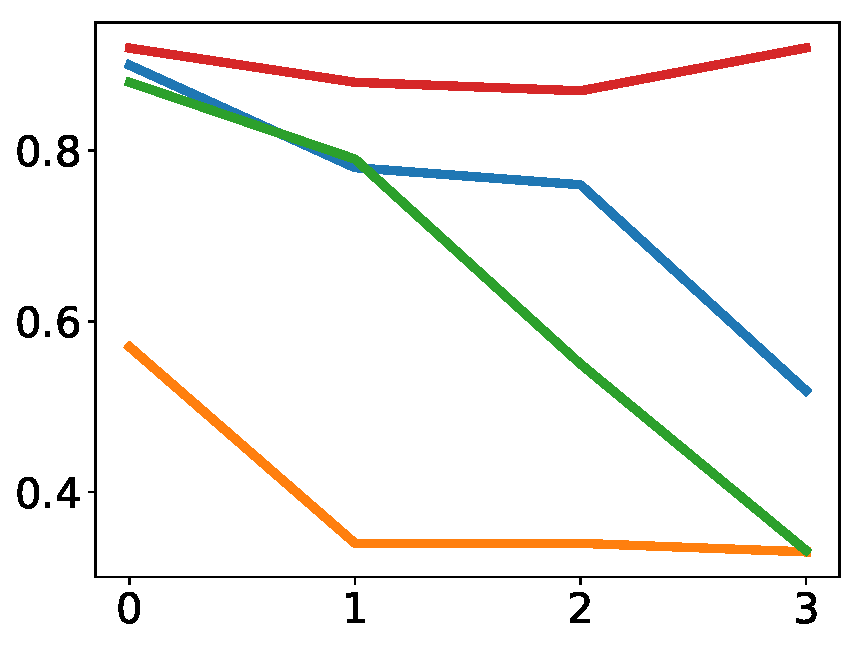
\includegraphics[width=0.24\textwidth]{figures/german-gender-f.pdf}
% 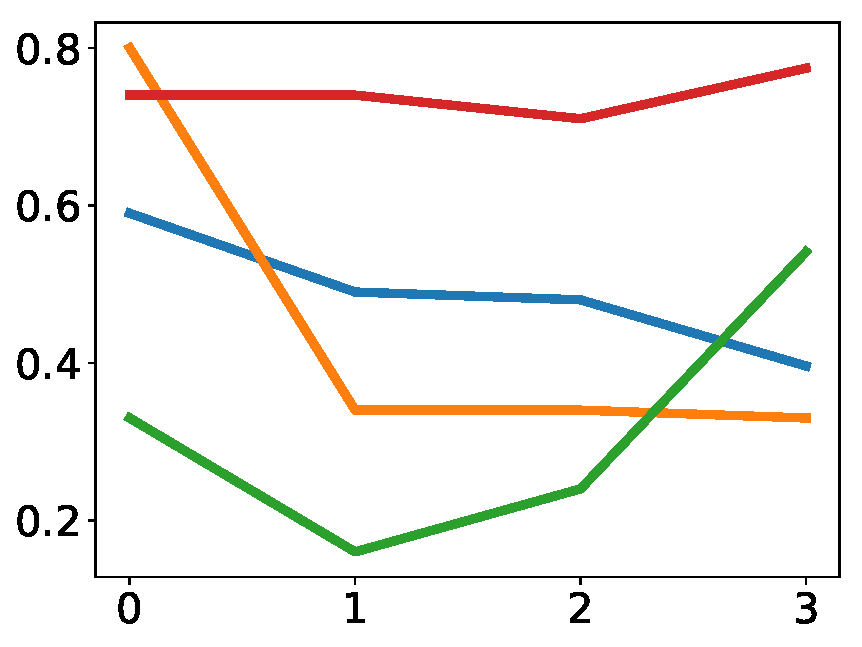
\includegraphics[width=0.24\textwidth]{figures/german-gender-n.pdf}
	\begin{tabular}{cccc}
		& Gender & Case & Subcategorization \\ 
		\raisebox{1.7\height}{\rotatebox[origin=c]{90}{Accuracy}}
		&
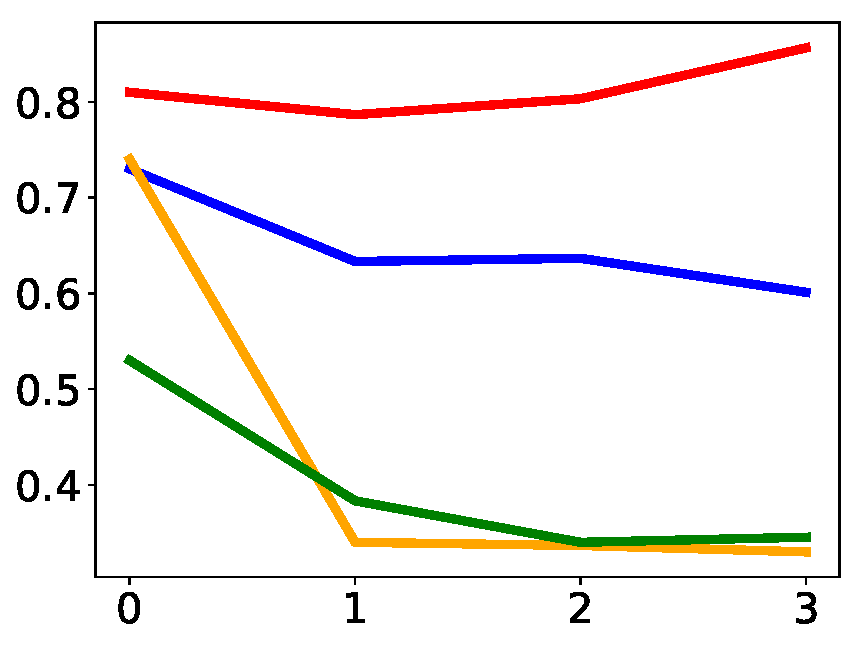
\includegraphics[width=0.28\textwidth]{figures/german-gender-total.pdf} 
		&
		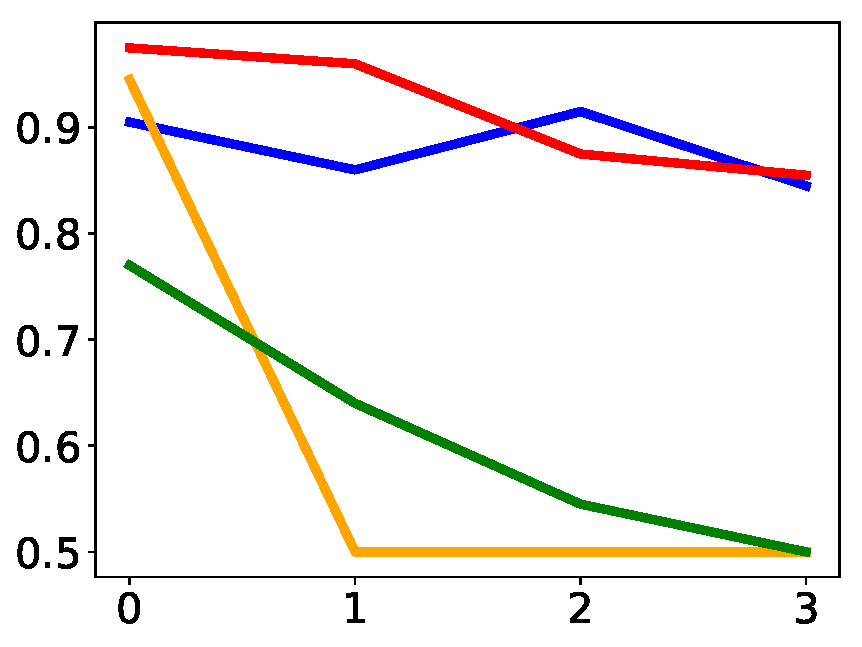
\includegraphics[width=0.28\textwidth]{figures/german-case-total.pdf}
		&
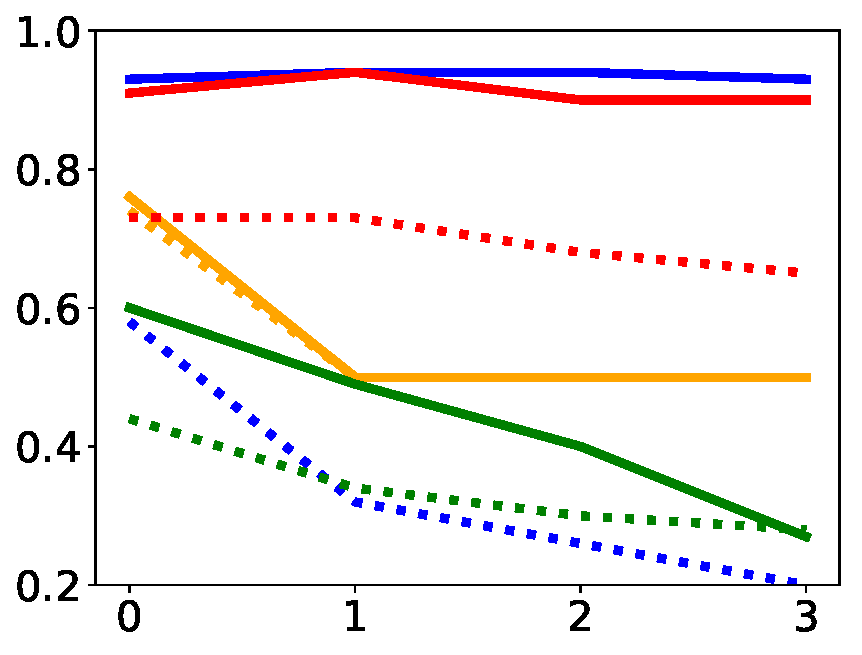
\includegraphics[width=0.28\textwidth]{figures/german-prep-with-control.pdf} \\ 
		&\multicolumn{3}{c}{Number of Intervening Words}
	\end{tabular}
\centering
\includegraphics[width=0.5\textwidth]{figures/german-legend.pdf}
\caption{Accuracy in the German syntax tasks, in function of number of intervening words.}\label{fig:german-syntax}
\end{figure*}

% \begin{figure*}
% % 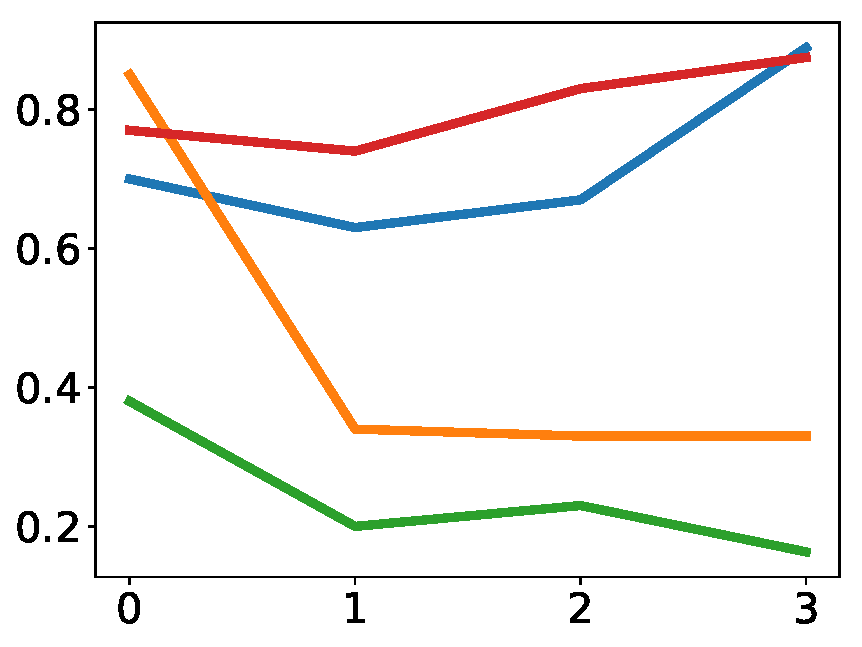
\includegraphics[width=0.24\textwidth]{figures/german-gender-m.pdf}
% % 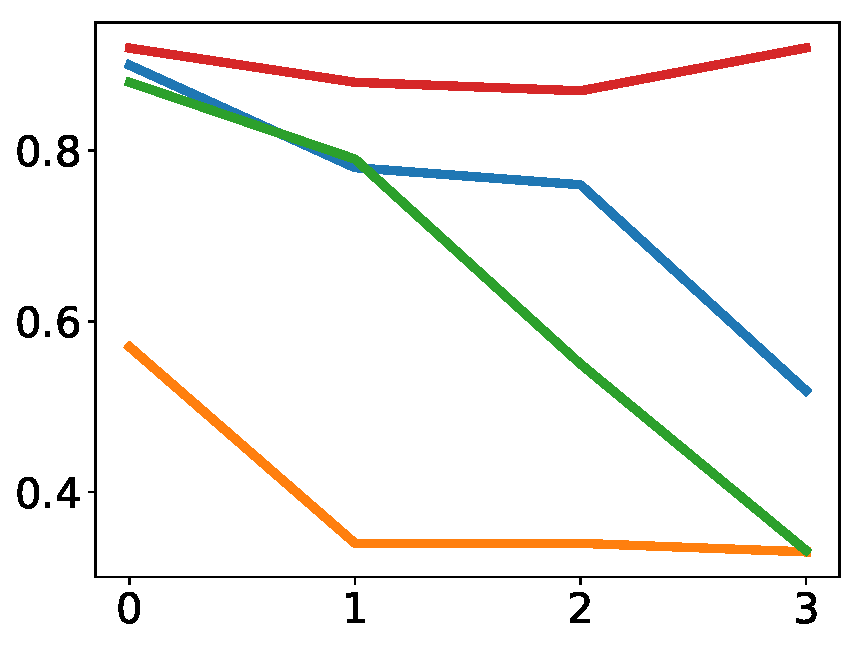
\includegraphics[width=0.24\textwidth]{figures/german-gender-f.pdf}
% % 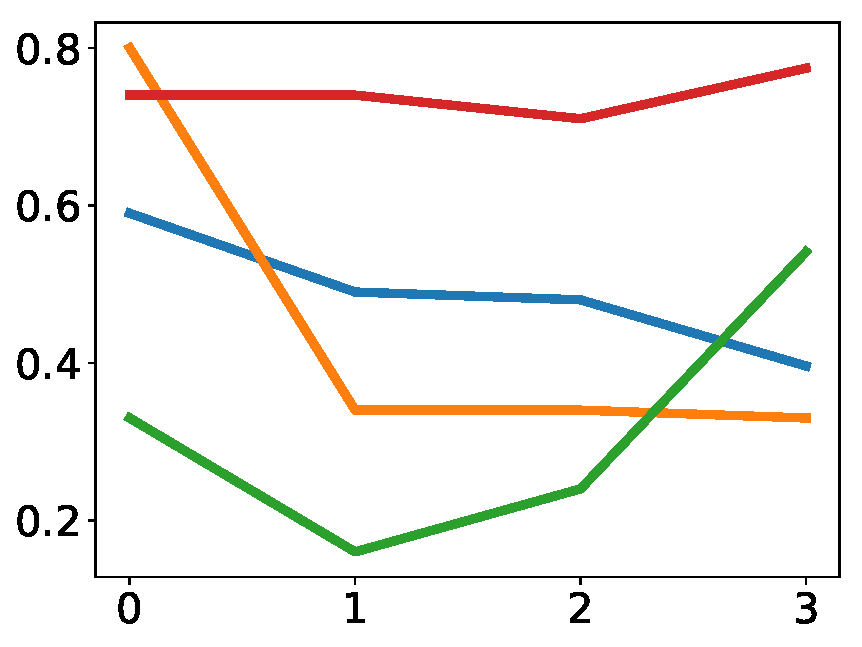
\includegraphics[width=0.24\textwidth]{figures/german-gender-n.pdf}
% 	\begin{tabular}{ccc}
% Gender & Case & Subcategorization \\
% 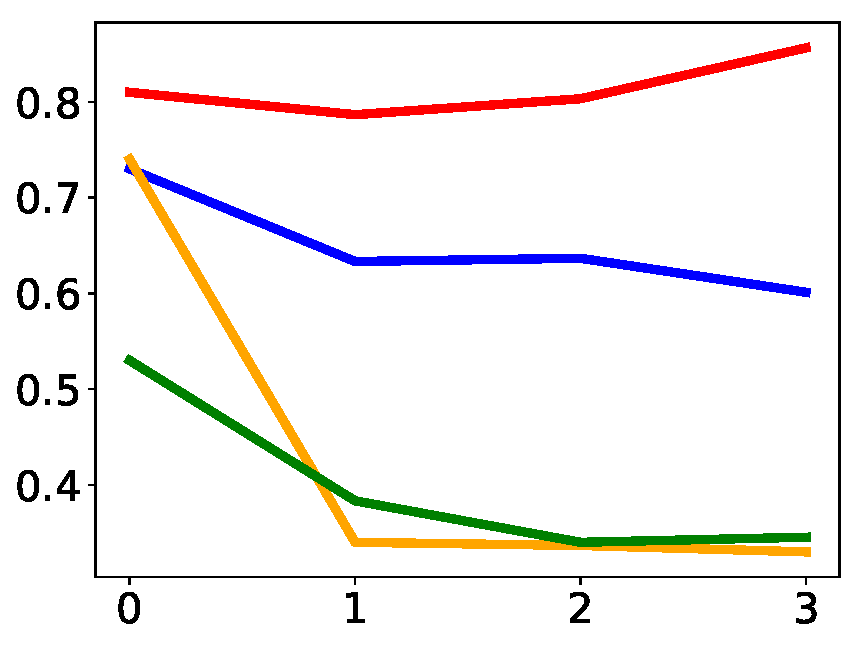
\includegraphics[width=0.33\textwidth]{figures/german-gender-total.pdf} 
% 		&
% 		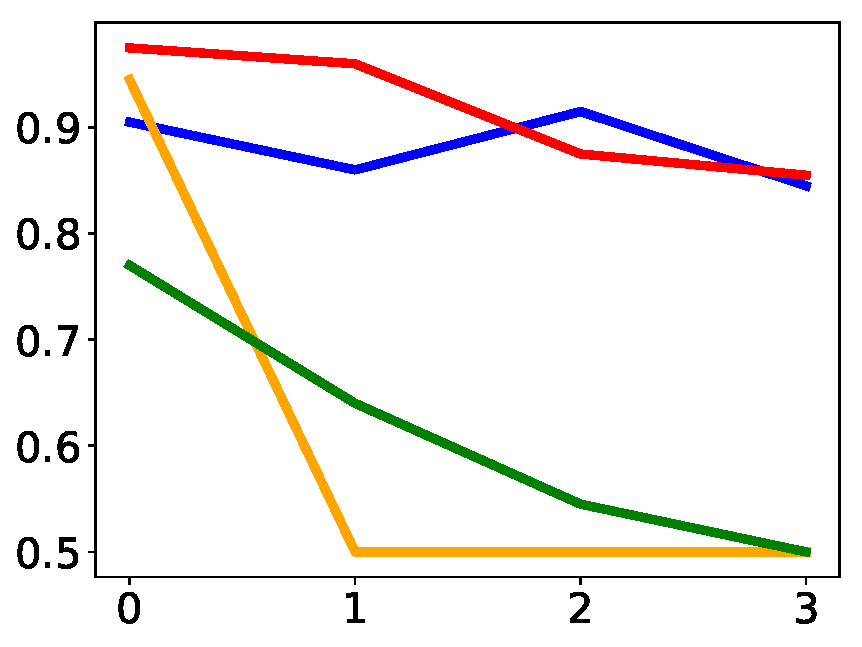
\includegraphics[width=0.33\textwidth]{figures/german-case-total.pdf}
% 		&
% 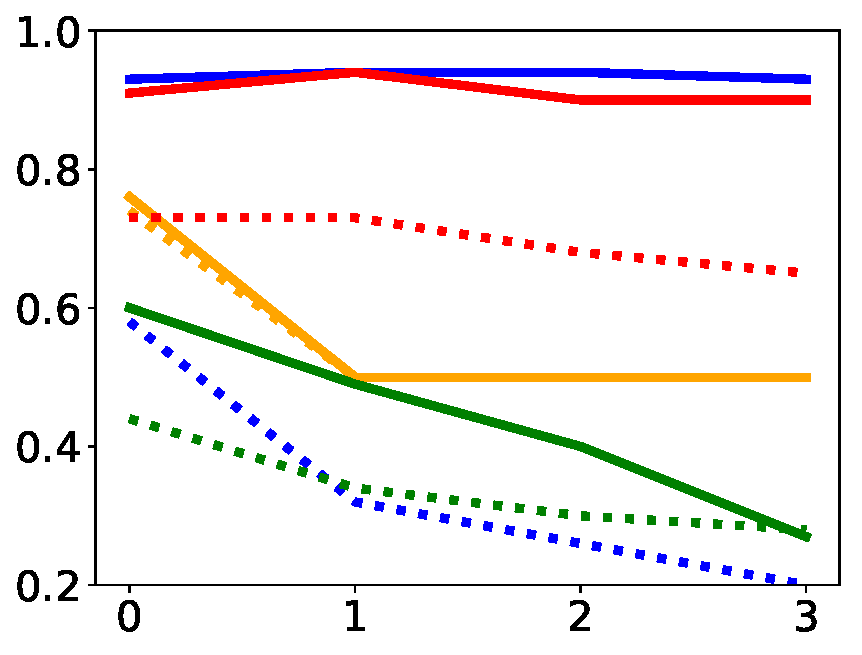
\includegraphics[width=0.33\textwidth]{figures/german-prep-with-control.pdf}
% 	\end{tabular}
% \centering
\includegraphics[width=0.5\textwidth]{figures/german-legend.pdf}
% \caption{Accuracy on the German syntax tasks, as a function of the number of intervening elements.}\label{fig:german-syntax}
% \end{figure*}


\paragraph{Article-noun case agreement}
We selected the two determiners \emph{dem} and \emph{des}, which
unambiguously indicate dative and genitive case, respectively, for
masculine and neuter nouns: %\textbf{Give one example.}
\ex.\ag. {\{\underline{dem}, des\}} sehr roten Baum \\
the very red {tree \emph{(dative)}} \\
\bg. {\{dem, \underline{des}\}} sehr roten Baums \\
the very red {tree \emph{(genitive)}} \\



%\begin{enumerate}[label={(\arabic*)}]
%	\item \begin{tabular}[t]{lllllll}
%	\{\underline{dem}, des\}& sehr& roten& Baum \\
%	article & adverb & adjective & noun \\
%	the & very & red & tree
%\end{tabular}
%\item \begin{tabular}[t]{lllllll}
%	\{dem, \underline{des}\}& sehr& roten& Baums \\
%	article & adverb & adjective & noun \\
%	the & very & red & tree
%\end{tabular}
%
%\end{enumerate}

We selected all noun lemmas of the appropriate genders from the German
UD treebank, and extracted morphological paradigms from Wiktionary to
obtain case-marked forms, retaining only nouns unambiguously marking
the two cases (4,509 nouns).  We created four conditions, varying the amount of
intervening material, as in the gender agreement experiment (4,509
stimuli per condition).  For 81.3\% of the nouns, at least one of the
two forms was OOV for the WordNLM, and we tested the latter on the
full-coverage subset.

Results are in Figure \ref{fig:german-syntax} (center).  Again,
WordNLM has the best performance, but the LSTM CNLM is competitive as
more elements intervene. Accuracy stays well above 80\% even with
three intervening words.  The n-gram model performs well if there is
no intervening material (again reflecting the obvious fact that
article-noun sequences are frequent in the corpus), and at chance
otherwise.  The RNN CNLM accuracy is above chance with one and two
intervening elements, but drops considerably with distance.

% Considering the results for the dative and genitive separately, accuracy slightly increases in the dative case and decreases in the genitive case.
% This can be attributed to the higher baseline frequency of dative in German, suggesting that both word- and character-based networks are impacted by unigram frequencies as more words intervene.
% This effect is far more pronounced for the RNN CNLM, explaining its overall decrease to chance level.
% Again, restricting to words that are in the word-level vocabulary did not change the pattern of results.
%\begin{figure}
%% 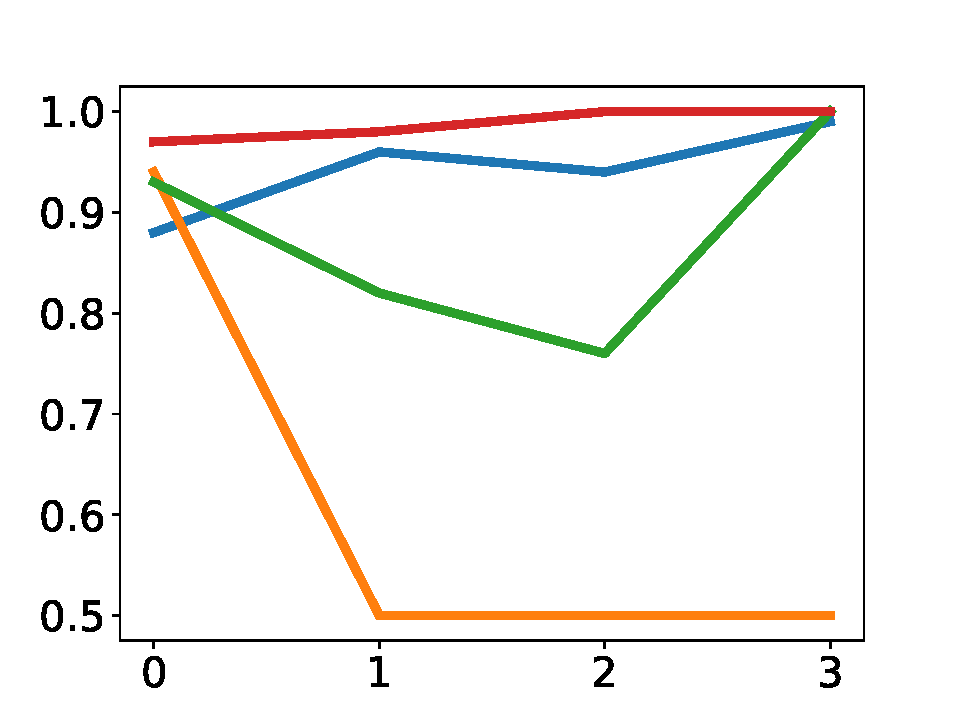
\includegraphics[width=0.23\textwidth]{figures/german-case-Dative.pdf}
%% 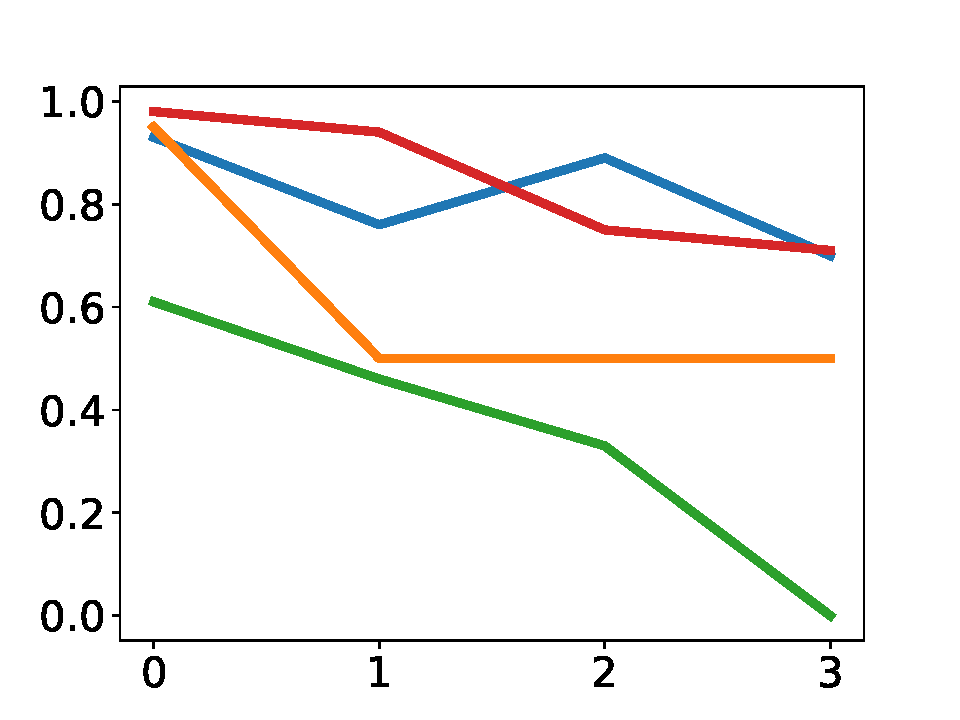
\includegraphics[width=0.23\textwidth]{figures/german-case-Genitive.pdf} \\
%
%\centering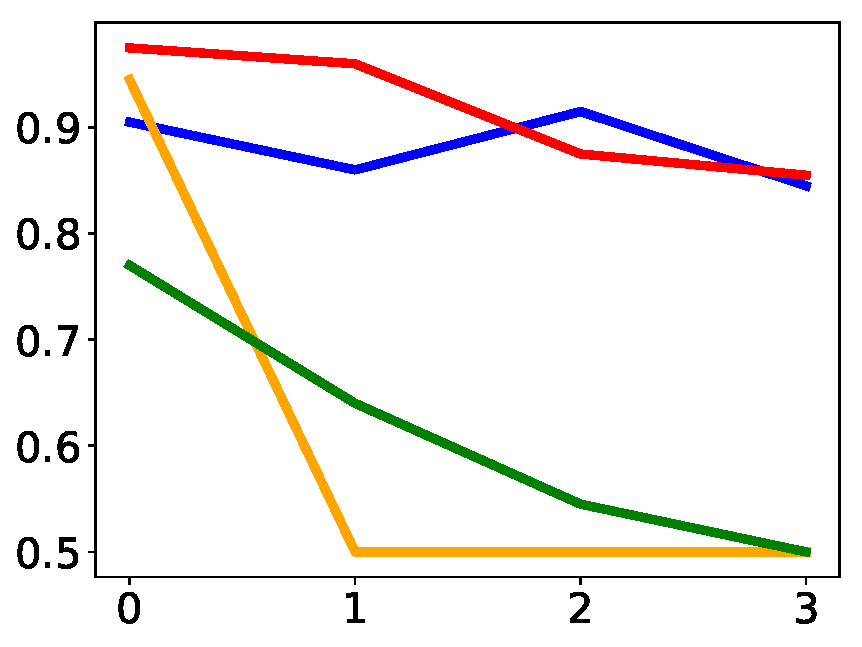
\includegraphics[width=0.24\textwidth]{figures/german-case-total.pdf}
%
%
\includegraphics[width=0.5\textwidth]{figures/german-legend.pdf}
%	\caption{\textbf{(Reduce to single figure, 2)} Accuracy on the case agreement task as a function of the number of intervening elements.}\label{fig:case}
%\end{figure}

\paragraph{Prepositional case subcategorization}
German verbs and prepositions lexically specify their object's case.  We
study the preposition \textit{mit} `with', which selects a dative
object. We focus on \textit{mit}, as it unambiguously requires a dative object,
and it is extremely frequent in the Wikipedia corpus we are using. To build the test set,
we select objects whose head noun is a nominalized adjective,
with regular, overtly marked case inflection.
We use the same adjective pool as in the preceding experiments.
%We take all adjectives
%that occur at least 100 times in the training data, excluding those
%that end in -\emph{r}, as these often reflected lemmatization
%problems.
We then select all sentences containing a \emph{mit} prepositional
phrase in the German Universal Dependencies treebank, subject to the
constraints that (1) the head of the noun phrase governed by the
preposition is not a pronoun (replacing such items with a nominal
object often results in ungrammaticality), and (2) the governed noun
phrase is continuous, in the sense that it is not interrupted by words
that do not belong to it.\footnote{The main source of noun phrase
  discontinuity in the German UD corpus is extraposition, a common
  phenomenon where part of the noun phrase is separated from the rest
  by the verb.} %\textbf{(please explain the latter more clearly)}.
We obtained 1,629 such sentences.  For each sentence, we remove the
prepositional phrase and replace it by a phrase of the form
\exg. mit der sehr \{rote,\ \underline{roten}\} \\
with the very red\ one \\

%\begin{enumerate}[label={(\arabic*)}]
%	\item \begin{tabular}[t]{lllllll}
%	mit & der & sehr& \{rote, \underline{roten}\} \\
%	prep & article  & adverb & adjective \\
%	with & the & very  & red one 
%\end{tabular}
%\end{enumerate}
where only the \emph{-en} (dative) version of the adjective is
compatible with the case requirement of the preposition (and the
intervening material does not disambiguate case). We construct three
conditions by varying the presence and number of adverbs (\emph{sehr}
`very', \emph{sehr extrem} `very extremely', \emph{sehr extrem
  unglaublich} `very extremely incredibly').  Note that here the
correct form is longer than the wrong one. As the overall likelihood
is the product of character probabilities ranging between 0 and 1, if
this introduces a length bias, it will work against the
character models. % ~\cite{sountsov2016length}.
Note also that we embed test phrases into full sentences (e.g., \emph{Die Figur hat \textbf{mit der roten} gespielt und meistens gewonnen.} `The figure played with the red one and mostly won'). We
do this as sentence-initial \emph{mit} is somewhat unnatural and, more
importantly, because this will disambiguate the final element of the
phrase as a noun (not an adjective), and exclude the reading in which
\emph{mit} is a particle not governing the noun phrase of
interest. When running the WordNLM, we excluded OOV adjectives as in
the previous experiments, but did not apply further OOV filtering to
the sentence frames.
% A full stimulus example with the wrapping sentence is:
% \exg. Die Figure hat mit der \{rote,\ \underline{roten}\} gespielt und meistens gewonnen . \\
% the figure has with the red\ one played and mostly won \\
% \textit{`The figure played with the red one and mostly won.'}

%\textbf{Add a full stimulus example (with the wrapping
%  sentence).} \textbf{OOV statistics.}



% Note also that in this case we embedded the test phrase into full sentences.
% We did this as sentences beginning with \emph{mit} are somewhat unnatural
% and, more importantly since \emph{mit} is homophonous with a particle
% that does not select for an object, and so that the following context disambiguates
% the last word in the phrase as a nominalization (as opposed to an adjective).

We also created control stimuli where all words up to and including
the preposition are removed (the example sentence above becomes:
\textit{der roten gespielt und meistens gewonnen}). If a model's
accuracy is lower on these control stimuli than on the full ones, its
performance cannot be simply explained by the different unigram
probabilities of the two adjective forms. For the n-gram baseline, we
only counted occurrences of the prepositional phrase, omitting the
sentential contexts.

%\begin{figure}
%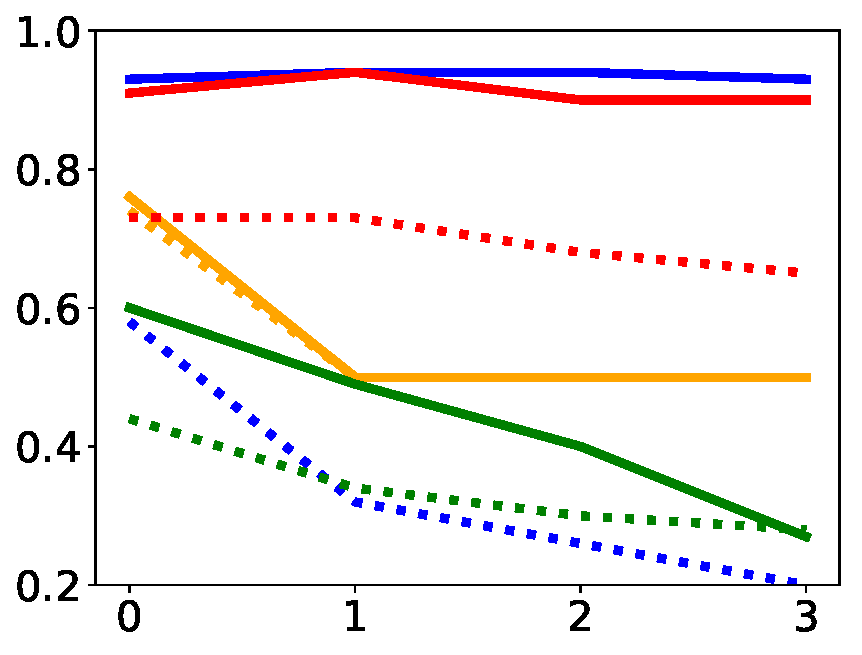
\includegraphics[width=0.48\textwidth]{figures/german-prep-with-control.pdf}
%
%
\includegraphics[width=0.48\textwidth]{figures/german-legend.pdf}
%\caption{\textbf{(Reduce to single figure, 3)} Accuracy on the subcategorization task as a function of the number of intervening elements. The dashed lines indicate accuracies on the control stimuli that do not contain the preposition.}\label{fig:prep}
%\end{figure}
%
Results are shown in Figure \ref{fig:german-syntax} (right). Only the
n-gram baseline fails to outperform control accuracy. Surprisingly,
the LSTM CNLM slightly outperforms the WordNLM, even though the latter
is evaluated on the easier full-lexical-coverage stimulus subset.
Neither model shows accuracy decay as the number of adverbs increases.
As before, the n-gram model drops to chance as adverbs intervene,
while the RNN CNLM starts with low accuracy that progressively decays
below chance.

%Results are shown in Table~\ref{tab:ital-agr-results}.
%The word LSTM shows the highest overall performance, closely followed by the LSTM CNLM.
%The RNN performs well on adjective gender, and considerably worse than the CNLM on the other tasks.
%For the CNLMs, the most challenging task was article-noun gender agreement.
%Discussion case-by-case, including how we control for n-gram frequency
%and length.
%Results table with a row for each pattern and a column for each model.

